%%  С точки зрения подачи информации было бы хорошо, где возможно, накрыть области, которые обсуждаем для библиотек
%%  
%%  ·        Анализ зрелости функционала и производительности библиотек на RISC-V
%%  
%%  ·        Готовность RISC-V для решения задач в выбранных областях, таких как (разреженная) линейная алгебра, граф аналитика, стандартизация тестирования свойств математических функций
%%  
%%  ·        Идентификация узких мест в выбранных алгоритмах, требующих аппаратной поддержки
%%  
%%  ·        Определение готовности стека ПО, необходимого для разработки высокопроизводительных библиотек (компиляторы, отладчики, профилировщики)
%%  
%%  ·        Формулировка предложений по развитию программно-аппаратного стека для выбранных областей
%%  
%%   
%%  
%%  На примере графов/разреженной алгебры/аппаратных расширений (все материалы есть):
%%  
%%  1)  граф аналитика: что это, почему, примеры задач/размерностей, примеры компаний, заинтересованных или предоставляющих решения
%%  
%%  2)  Зрелость функциональной области:
%%  
%%            - GraphBLAS, связка с разреженной линейной алгеброй, его множественные реализации для не RISC-V
%%  
%%            - наборы стандартных датасетов
%%  
%%            - степень стандартизации по теме
%%  
%%  3) Зрелость стека:
%%  
%%        - компиляторы, функциональная эмуляция, отладка, профилировка, время сборки, время запусков итп
%%  
%%        - вычислительный патерн, оптимизации под существующее железе
%%  
%%  4)   Зрелость железа:
%%  
%%         - RVV
%%  
%%         - существующие предложения по расширениям, приоритеты
%%  
%%         - GPU вкл Vortex
%%  
%%         - доступность железа
%%  
%%  5) Подмножества измерений
%%  
%%  6) Выводы о готовности, возможностях оптимизаций в рамках существующего функционала аппаратуры, следующие шаги
%%  
%%   
%%  
%%  При этом хотим вписаться в 25 мин + 5 мин на вопросы
%%  
%%  Имеет смысл?
%20 min preso!
\documentclass[xcolor=table,aspectratio=169]{beamer}
\usepackage{beamerthemesplit}
\usepackage{wrapfig}
\usetheme{SPbGU}
\usepackage{pdfpages}
\usepackage{amsmath}
\usepackage{cmap}
\usepackage[T2A]{fontenc}
\usepackage[utf8]{inputenc}
\usepackage[english]{babel}
\usepackage{indentfirst}
\usepackage{amsmath}
\usepackage{tikz}
\usepackage{multirow}
\usepackage[noend]{algpseudocode}
\usepackage{algorithm}
\usepackage{algorithmicx}
\usepackage{fancyvrb}
\usepackage{hyperref} 
\definecolor{links}{HTML}{2A1B81}
\hypersetup{colorlinks,linkcolor=,urlcolor=links}
\usetikzlibrary{calc}
\usetikzlibrary{shapes, backgrounds}
\usetikzlibrary{arrows,automata}
\usetikzlibrary{positioning}
\usetikzlibrary{fit}
\usetikzlibrary{shapes.callouts}
\usetikzlibrary{shapes.misc}
\usepackage{xparse}
\usepackage{fontawesome}

\usepackage{etoolbox,refcount}
\usepackage{multicol}

\usepackage{tabularx}
\newcolumntype{Y}{>{\raggedleft\arraybackslash}X}

\renewcommand{\thealgorithm}{}

\newtheorem{mytheorem}{Theorem}
\renewcommand{\thealgorithm}{}

\newcommand{\tikzmark}[1]{\tikz[overlay,remember picture] \node (#1) {};}
\def\Put(#1,#2)#3{\leavevmode\makebox(0,0){\put(#1,#2){#3}}}

\newcommand{\ltz}{$< 1$}

\tikzset{
    state/.style={
           rectangle,
           rounded corners,
           draw=black, very thick,
           minimum height=2em,
           inner sep=2pt,
           text centered,
           },
}

\tikzset{
    invisible/.style={opacity=0,text opacity=0},
    visible on/.style={alt=#1{}{invisible}},
    alt/.code args={<#1>#2#3}{%
      \alt<#1>{\pgfkeysalso{#2}}{\pgfkeysalso{#3}} % \pgfkeysalso doesn't change the path
    },
}

\tikzset{cross/.style={cross out, draw=black, minimum size=2*(#1-\pgflinewidth), inner sep=0pt, outer sep=0pt, ultra thick},
%default radius will be 1pt. 
cross/.default={1pt}}

\NewDocumentCommand{\mycallout}{r<> O{opacity=0.8,text opacity=1} m m m}{%
\tikz[remember picture, overlay]\node[align=center, fill=cyan!20, text width=#5cm,
#2,visible on=<#1>, rounded corners,
draw,rectangle callout,anchor=pointer,callout relative pointer={(290:0.5cm)}]
at (#3) {#4};
}

\NewDocumentCommand{\mycalloutR}{r<> O{opacity=0.8,text opacity=1} m m m}{%
\tikz[remember picture, overlay]\node[align=center, fill=cyan!20, text width=#5cm,
#2,visible on=<#1>, rounded corners,
draw,rectangle callout,anchor=pointer,callout relative pointer={(30:0.8cm)}]
at (#3) {#4};
}

\newcommand\colR{\cellcolor{red!20}}
\newcommand\colB{\cellcolor{blue!20}}
\newcommand\colG{\cellcolor{green!20}}

%callout relative pointer={(230:0.5cm)}]
\setbeamertemplate{page number in head/foot}[appendixframenumber]
\newcounter{countitems}
\newcounter{nextitemizecount}
\newcommand{\setupcountitems}{%
  \stepcounter{nextitemizecount}%
  \setcounter{countitems}{0}%
  \preto\item{\stepcounter{countitems}}%
}
\makeatletter
\newcommand{\computecountitems}{%
  \edef\@currentlabel{\number\c@countitems}%
  \label{countitems@\number\numexpr\value{nextitemizecount}-1\relax}%
}
\newcommand{\nextitemizecount}{%
  \getrefnumber{countitems@\number\c@nextitemizecount}%
}
\newcommand{\previtemizecount}{%
  \getrefnumber{countitems@\number\numexpr\value{nextitemizecount}-1\relax}%
}
\makeatother    
\newenvironment{AutoMultiColItemize}{%
\ifnumcomp{\nextitemizecount}{>}{3}{\begin{multicols}{2}}{}%
\setupcountitems\begin{itemize}}%
{\end{itemize}%
\unskip\computecountitems\ifnumcomp{\previtemizecount}{>}{3}{\end{multicols}}{}}


\beamertemplatenavigationsymbolsempty

\title[GraphBLAS на RISC-V]{Анализ графов и разреженная линейная алгебра в экосистеме RISC-V}
\subtitle{Рабочая группа ``Развитие экосистемы ПО на RISC-V''}
\institute[СПбГУ]{
Санкт-Петербургский Государственный Университет
}

% То, что в квадратных скобках, отображается в левом нижнем углу.
\author[Семён Григорьев]{Семён Григорьев}

\date{3 октября 2025}

\begin{document}
{
\begin{frame}[fragile]
  \begin{table}
  \centering
  %
\includegraphics[height=1.5cm]{pictures/SPbGU_Logo.png}
  \begin{tabularx}{\linewidth}{XcX}
    %
\includegraphics[height=0.9cm]{pictures/hu_logo.jpeg} 
    \hfill
    & 
    & \hfill 
\includegraphics[height=1.6cm]{pictures/SPbGU_Logo.png}
  \end{tabularx}
  \end{table}
  \titlepage
\end{frame}
}

\begin{frame}[fragile]
  \frametitle{Линейная алгебра и анализ графов: области применения}
  \begin{itemize}
    \item \textbf{Анализ больших графов}: графовые БД, анализ кода, поиск уязвимостей, анализ трафика, анализ транзакцйи, банковская аналитика, социальные сети\ldots
      \begin{itemize}        
        \item Важна производительность
        \item \underline{\textbf{Разнообразные алгоритмы}}        
      \end{itemize}
    \item Разреженная обощённая линейная алгебра --- путь к \underline{\textbf{унифицированной}} параллельной обработке графов 
    \item Примеры заинтересованных сторон
      \begin{itemize}
        \item Sber и \href{https://cdn-app.sberdevices.ru/misc/0.0.0/assets/common/825c0d52_1_bulavin_slide.pdf}{Montecristo}
        \item VK и \href{https://habr.com/ru/companies/vk/articles/665156/}{Tarantool}
        \item ИТ-холдинг Т1 и \href{https://habr.com/ru/companies/T1Holding/articles/755174/}{Мирион}
        \item \href{https://highload.ru/spb/2025/abstracts/14537}{Т-Банк}
        \item \ldots
      \end{itemize}
    \end{itemize}
\end{frame}

\begin{frame}[fragile]
  \frametitle{Линейная алгебра и анализ графов: особенности}
  
    \begin{itemize}
      \item \textbf{Обобщённая}: матрицы и вектора параметризованы типом элемента, операции над ними могут быть заданы пользователем
        \begin{itemize}
          \item Нет фиксированного набора типов и операций
        \end{itemize}
      \item \textbf{Разреженная}: специализированные структуры для хранения матриц и векторов с малым числом значимых элементов, специализированные алгоритмы для их обработки 
      \begin{itemize}
          \item Понимание разреженности различается от области к области: для AI/ML типично заполнение \underline{десятков процентов} ячеек, для графов --- \underline{много меньше $1\%$}        
        \end{itemize}
        \item \textbf{Не все решения, удачные для AI/ML и вычислительной математики окажутся удачными для анализа графов}\footnote{RVV, матричные расширения и т.д.}
    \end{itemize}
\end{frame}

\begin{frame}[fragile]
  \frametitle{GraphBLAS API\footnote{\url{https://graphblas.org/}}}
  \begin{itemize}
    \item API для создания алгоритмов анализа графов на основе линейной алгебры 
    \begin{itemize}
      \item Различные операции над матрицами и векторами (\underline{\textbf{разреженными}})
      \item Параметризация алгебраическими структурами: полукольцами, моноидами и т.д.
    \end{itemize}
    \item Выразимы \underline{\textbf{различные}} алгоритмы (в LAGraph \underline{\textbf{более 20 различных задач}})
    \begin{itemize}
      \item Обход в ширину, поиск кратчайших путей, достижимость, \ldots
      \item Подсчёт треугольников, PageRank, остовные деревья, кластеризация,\ldots
      \item Запросы с регулярными (RPQ) и контекстно-свободными (CFPQ) ограничениями \ldots      
    \end{itemize}
    \item Подробнее
    \begin{itemize}
      \item The GraphBLAS C API Specification\footnote{\url{https://graphblas.org/docs/GraphBLAS_API_C_v2.1.0.pdf}}
      \item GraphBLAS Pointers\footnote{\url{https://graphblas.org/GraphBLAS-Pointers/}}
      \item Introduction to GraphBLAS\footnote{\url{https://zenodo.org/record/4318870/files/graphblas-introduction.pdf}}
      \item LAGraph\footnote{\url{https://github.com/GraphBLAS/LAGraph}}
    \end{itemize}
    \end{itemize}
\end{frame}

\begin{frame}[fragile]
  \frametitle{Реализации GraphBLAS-подобных API}
  \begin{itemize}
      \item \textbf{SuiteSparse:GraphBLAS}\footnote{\url{https://github.com/DrTimothyAldenDavis/GraphBLAS}}: \underline{\textbf{эталон}} на чистом C
      \begin{itemize}
        \item Используется в \href{https://networkx.org/}{NetworkX}, \href{https://www.falkordb.com/}{FalkorDB}, \href{https://onesparse.com/}{OneSparse}, \href{https://www.open3d.org/}{Open3d}, \href{http://eigen.tuxfamily.org/}{Eigen}, \href{https://octave.org/}{GNU Octave} и т.д.
        \item Ведутся работы по использованию GPU через Cuda
        \item Обёртки для различных языков: Python, Rust, \ldots
      \end{itemize}
      \item Huawei's GraphBLAS\footnote{\url{https://gitee.com/CSL-ALP/graphblas}}: частичная реализация на C++
      \item CombBLAS\footnote{\url{https://github.com/PASSIONLab/CombBLAS}}: распределённая, частичная реализация на C++
      \item GraphBLAST\footnote{\url{https://github.com/gunrock/graphblast}}: поддержка GPGPU, Cuda C, частичная реализация
      \item \textbf{Spla}\footnote{\url{https://github.com/SparseLinearAlgebra/spla}}: поддержка GPGPU, OpenCL C, частичная реализация
      \item GraphLily\footnote{\href{https://dl.acm.org/doi/10.1109/ICCAD51958.2021.9643582}{GraphLily: Accelerating Graph Linear Algebra on HBM-Equipped FPGAs}}: подмножество GraphBLAS на FPGA      
  \end{itemize}
\end{frame}

\begin{frame}[fragile]
  \frametitle{Наборы данных и бенчмарки}
  \begin{itemize}
    \item \href{https://ldbcouncil.org/benchmarks/overview/}{Linked Data Benchmark Council (LDBC)}
      \begin{itemize}
        \item \href{https://ldbcouncil.org/benchmarks/graphalytics/}{LDBC Graphalytics Benchmark}: алгоритмы анализа графов
        \item \href{https://ldbcouncil.org/benchmarks/spb/}{LDBC Semantic Publishing Benchmark}: семантические сети (RDF)
        \item \ldots
      \end{itemize}
      \item \href{http://sparse.tamu.edu/}{Suite Sparse Matrix Collection}: набор разреженных матриц различной природы
      \begin{itemize}
        \item В LAGraph есть \href{https://github.com/GraphBLAS/LAGraph/tree/stable/src/benchmark}{своя инфраструктура для экспериментов}
      \end{itemize}
      \item \href{https://graph500.org/?page_id=12}{Graph500}: алгоритмы анализа графов для суперкомпьютеров
      \item \href{http://gap.cs.berkeley.edu/benchmark.html}{GAP}: алгоритмы анализа графов
      \item \ldots
  \end{itemize}
\end{frame}

\begin{frame}[fragile]
  \frametitle{SuiteSparse:GraphBLAS на RISC-V}
  \begin{itemize}
      \item SuiteSparse:GpaphBLAS (и SuiteSparse целиком) готов к использованию на RISC-V
    \begin{itemize}
      \item[\faCheck] Кросс-сборка: 12мин. на Intel Core i5-1340P, 4х4.6ГГц, 8х3.4ГГц
      \item[\faCheck] Нативно: 1ч.48мин. на Milk-V (8 ядер 1.6 ГГц)
      \item[\faCheck] Тесты проходят
      \item[\faCheck] Поддержка RISC-V в CI есть\footnote{Соответствующий реквекст: \url{https://github.com/DrTimothyAldenDavis/SuiteSparse/pull/949}}
    \end{itemize}
    \vfill
    \item Есть простор для оптимизаций
    \begin{itemize}
      \item Ручная векторизация\footnote{Есть поддержка AVX и Neon, а с RVV1.0 только эксперименты: \url{https://github.com/DrTimothyAldenDavis/GraphBLAS/pull/381}}
      \item Изучение возможностей автоматической векторизации\footnote{В проекте много кода, написанного с расчётом на автоматическую векторизацию}
      \item Применимость матричных расширений\footnote{На текущий момент они нацелены на AI/ML, а это другое}
    \end{itemize}  
  \end{itemize}
\end{frame}

\begin{frame}[t]
  \frametitle{Результаты векторизации умножения матриц в SuiteSparse:GraphBLAS\footnote{\textbf{SoC}: SPACEMIT K1/M1, Octa-core X60™(RV64GCVB), 1.6GHz, RVA22, RVV1.0}}
  \begin{center}
    \resizebox{0.9\textwidth}{!}{
    \tikzmark{zzz}{ }
    \begin{tabular}{|p{0.5cm}|p{3.4cm}|p{1.4cm}|p{1.5cm}|p{1.3cm}|p{1.3cm}|p{1.5cm}|p{1.5cm}|p{1.28cm}|p{1.28cm}|}
        \hline
        \textbf{№} & \textbf{Matrix name} & \textbf{Rows number} & \textbf{Nonzeros}& \textbf{AVX2 (ms.)}& \textbf{No AVX2 (ms.)}& \textbf{RVV (ms.)}& \textbf{No RVV (ms.)}& \textbf{AVX speedup (\%)}& \textbf{RVV speedup (\%)} \\
        \hline
        1 & olafu & 16146 & 515651 & 5327.7 & 6629.7 & 43080.7 & 52940.1 & 19.6 & \cellcolor{green!25}18.6 \\
        \hline
        \cellcolor{ red!30}2 & \cellcolor{red!30}fd18 & \cellcolor{red!30}16428 & \cellcolor{red!30}63406 & \cellcolor{red!30}476.4 & \cellcolor{red!30}482.0 & \cellcolor{red!30}2212.6 & \cellcolor{red!30}2181.2 & \cellcolor{red!30}1.2 & \cellcolor{red!50}-1.4 \\
        \hline
        3 & sme3Da & 12504 & 874887 & 4236.9 & 5124.9 & 32008.0 & 42763.8 & 17.3 & \cellcolor{green!25}25.2 \\
        \hline
        4 & stokes64 & 12546 & 74242 & 508.8 & 564.4 & 2629.7 & 2814.1 & 9.8 & \cellcolor{green!25}6.6\\
        \hline
        5 & sinc12 & 7500 & 294986 & 632.6 & 864.0 & 5970.1 & 8593.8 & 26.8 & \cellcolor{green!25}30.5\\
        \hline
        6 & fd12 & 7500 & 28462 & 90.4 & 92.3 & 484.1 & 555.3 & 2.0 & \cellcolor{green!25}12.8\\
        \hline
        7 & bcsstk15 & 3948 & 60882 & 87.8 & 117.9 & 1271.5 & 1770.8 & 25.6 & \cellcolor{green!25}28.2\\
        \hline
        8 & tols4000 & 4000 & 8784 & 17.1 & 18.2 & 184.0 & 203.5 & 5.9 & \cellcolor{green!25}9.6\\
        \hline
        9 & ex36 & 3079 & 53843 & 28.5 & 41.0 & 574.2 & 584.8 & 30.5 & \cellcolor{green!25}1.8\\
        \hline
        10 & iprob & 3001 & 9000 & 25.2 & 34.7 & 279.3 & 344.9 & 27.5 & \cellcolor{green!25}19.0\\
        \hline
        11 & MISKnowledgeMap & 2427 & 28511 & 31.3 & 38.5 & 401.6 & 490.0 & 18.8 & \cellcolor{green!25}18.0 \\
        \hline
        \cellcolor{ red!30}12 & \cellcolor{ red!30}LeGresley\_2508 & \cellcolor{ red!30}2508 &\cellcolor{ red!30}16727 & \cellcolor{ red!30}10.4 & \cellcolor{ red!30}12.1 & \cellcolor{ red!30}106.5 & \cellcolor{ red!30}97.7 & \cellcolor{ red!30}14.3 & \cellcolor{red!50}-8.9\\
        \hline
        13 & reorientation\_2 & 1544 & 9408 & 5.6 & 9.8 & 117.9 & 125.4 & 42.7 & \cellcolor{green!25}6.0\\
        \hline
        \cellcolor{ red!30}14 & \cellcolor{ red!30}netscience & \cellcolor{ red!30}1589 & \cellcolor{ red!30}2742 & \cellcolor{ red!30}1.5 & \cellcolor{ red!30}2.8 & \cellcolor{ red!30}31.4 & \cellcolor{ red!30}28.5 & \cellcolor{ red!30}47.0 & \cellcolor{red!50}-10.0\\
        \hline
        15 & mcfe & 765 & 24382 &2.3 & 5.5 & 51.1 & 65.3 & 58.8 & \cellcolor{green!25}21.8\\
        \hline
        16 & orbitRaising\_3 & 761 & 3256 & 0.6 & 1.6 & 10.5 & 13.1 & 63.0 & \cellcolor{green!25}19.5\\
        \hline

    \end{tabular}
}
  \end{center}
  %\onslide<2>{
    \tikz[overlay,remember picture]{\draw[draw=blue,thick,double,fill opacity=0.2] ($ (zzz) + (11.1,0.6)$) rectangle ($ (zzz) + (13.5,0.25)$);}
    \tikz[overlay,remember picture]{\draw[draw=blue,thick,double,fill opacity=0.2] ($ (zzz) + (11.1,1.6)$) rectangle ($ (zzz) + (13.5,1.25)$);}
   % }
  %\onslide<3>{
    \tikz[overlay,remember picture]{\draw[draw=red,thick,double,fill opacity=0.2] ($ (zzz) + (11.1,-2.45)$) rectangle ($ (zzz) + (13.5,-3.15)$);}
    \tikz[overlay,remember picture]{\draw[draw=red,thick,double,fill opacity=0.2] ($ (zzz) + (11.1,-0.43)$) rectangle ($ (zzz) + (13.5,-0.75)$);}
    \tikz[overlay,remember picture]{\draw[draw=red,thick,double,fill opacity=0.2] ($ (zzz) + (11.1,-1.8)$) rectangle ($ (zzz) + (13.5,-2.14)$);}
  %  }
\end{frame}

\begin{frame}[fragile]
  \frametitle{RISC-V и GPGPU}
  \begin{itemize}
    \item \textbf{RISC-V CPU + Imagination Technologies GPU}: самая распространённая (из доступных) конфигурация
    \item \textbf{RISC-V CPU + AMD GPU}: утверждается, что работает и есть официальная поддержка (\href{https://milkv.io/pioneer}{Milk-V Pioneer}, \href{https://riscv.org/ecosystem-news/2024/10/risc-v-cpu-demoed-with-rx-7900-xtx-gpu-in-debian-linux-amd-flagship-gpu-paired-with-milk-v-megrez-board-and-sifive-p550-cores/}{Milk-V Megrez}, \href{https://milkv.io/ruyibook}{RuyiBook})
    \item \textbf{RISC-V CPU + Intel GPU}: \href{https://www.reddit.com/r/RISCV/comments/1ftep9u/intel_arc_a770_on_riscv/}{ходят слухи, что можно}, но официальной поддержки пока нет
    \item \textbf{RISC-V CPU + Nvidia GPU}: \href{https://riscv.org/ecosystem-news/2025/07/nvidia-to-bring-cuda-platform-support-to-the-risc-v/}{анонсировано}
    \item \textbf{RISC-V GPU}: \href{https://github.com/vortexgpgpu/vortex}{Vortex} (только на ПЛИС)
  \end{itemize}
\end{frame}

\begin{frame}[fragile]
  \frametitle{Spla на RISC-V}
  \begin{itemize}
    \item[\faCheck] \textbf{RISC-V CPU + Imagination Technologies GPU}: собирается, запускается, тесты проходят
    \item[\faGears] \textbf{RISC-V GPU Vortex}: собирается, запускается, не все тесты проходят    
    \item[\faHourglassHalf] \textbf{RISC-V CPU + AMD GPU, Intel GPU, Nvidia GPU}: требуется проверка
    \begin{itemize}
      \item Cерьёзных проблем не ожидается, так как на аналогичных конфигурациях с x86 CPU всё нормально\footnote{Разве что на уровне драйвера или другого системного ПО, не относящегося к библиотеке}
    \end{itemize}
    \vfill
    \item Есть простор для оптимизаций
    \begin{itemize}
      \item Performance Portability Problem никто не отменял
      \item Эксперименты с различными конфигурациями Vortex      
    \end{itemize}
    \item Vortex пока относительно ``сырой''
    \begin{itemize}
      \item \href{https://github.com/vortexgpgpu/vortex/issues/251}{Проблемы со сбросом регистров}
      \item Проблемы с работой с памятью (не все функции для \texttt{clBuffer} работают)
      \item Проблемы с ``сервисными'' функциями (типа \texttt{getProgramInfo})
      \item \ldots
    \end{itemize}
  \end{itemize}
\end{frame}

\begin{frame}
  \frametitle{Spla на SpacemiT M1 CPU, IMG BXE-2-32 GPU}

\begin{columns}
        \column{0.5\textwidth}        
        \vspace{-0.5cm}
        \begin{center}
          BFS \\
        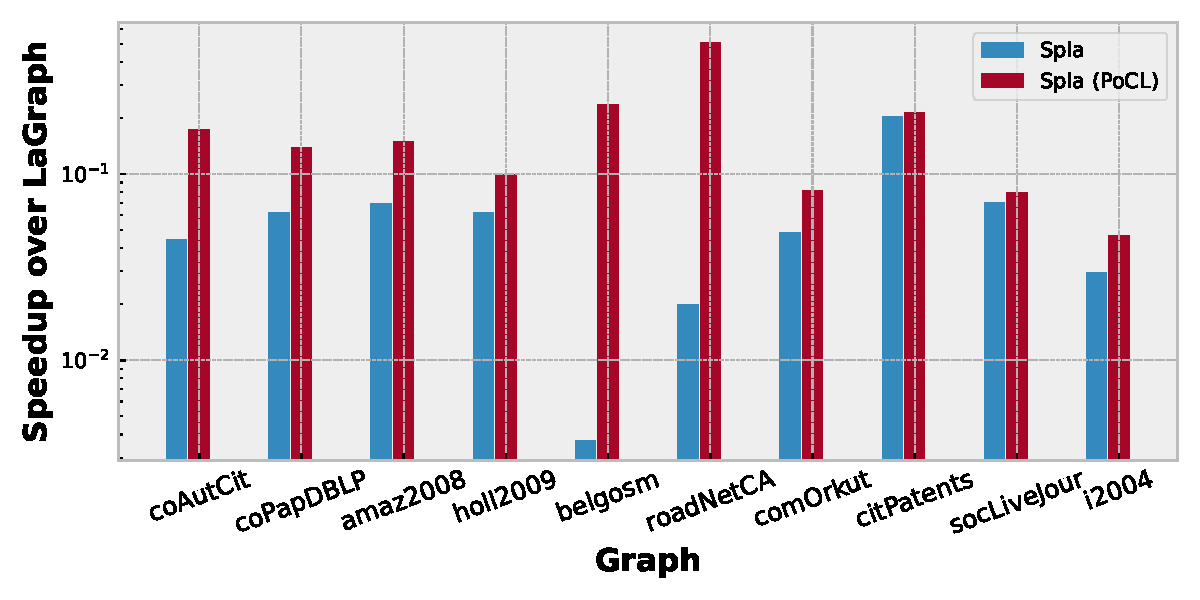
\includegraphics[width=0.909\linewidth]{pictures/rq1_rel_bfs.pdf}
        Single Source Shortest Path (SSSP) \\
        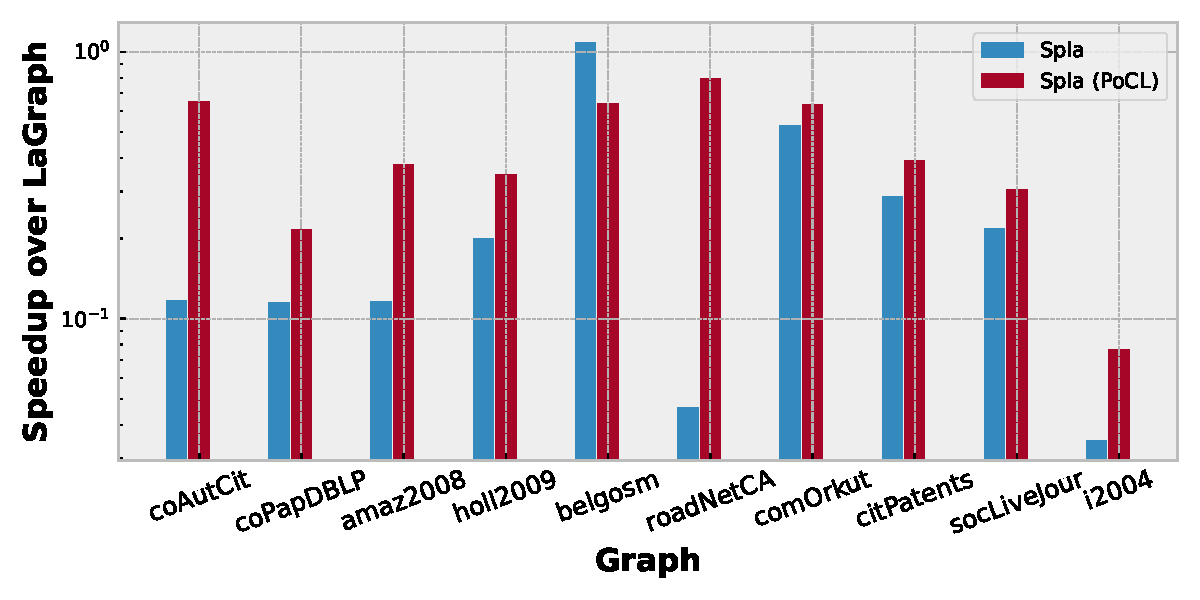
\includegraphics[width=0.909\linewidth]{pictures/rq1_rel_sssp.pdf}
        \end{center}
        \column{0.5\textwidth}
        \vspace{-0.5cm}
        \begin{center}
          Triangle Count (TC) \\
        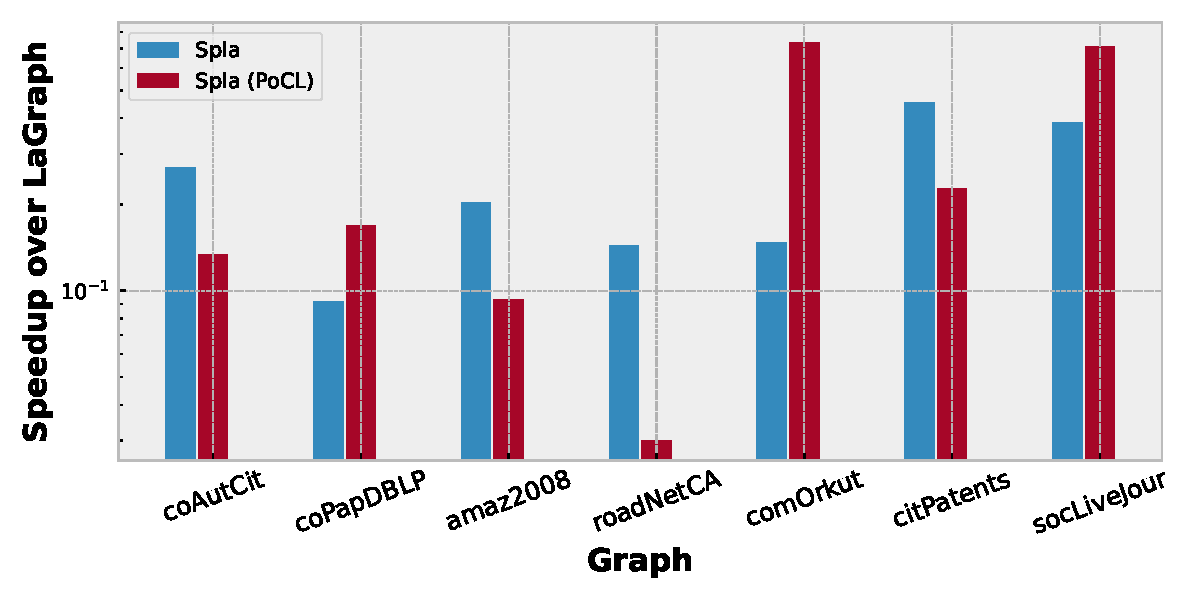
\includegraphics[width=0.9\linewidth]{pictures/rq1_rel_tc.pdf}
        PageRank (PR) \\
        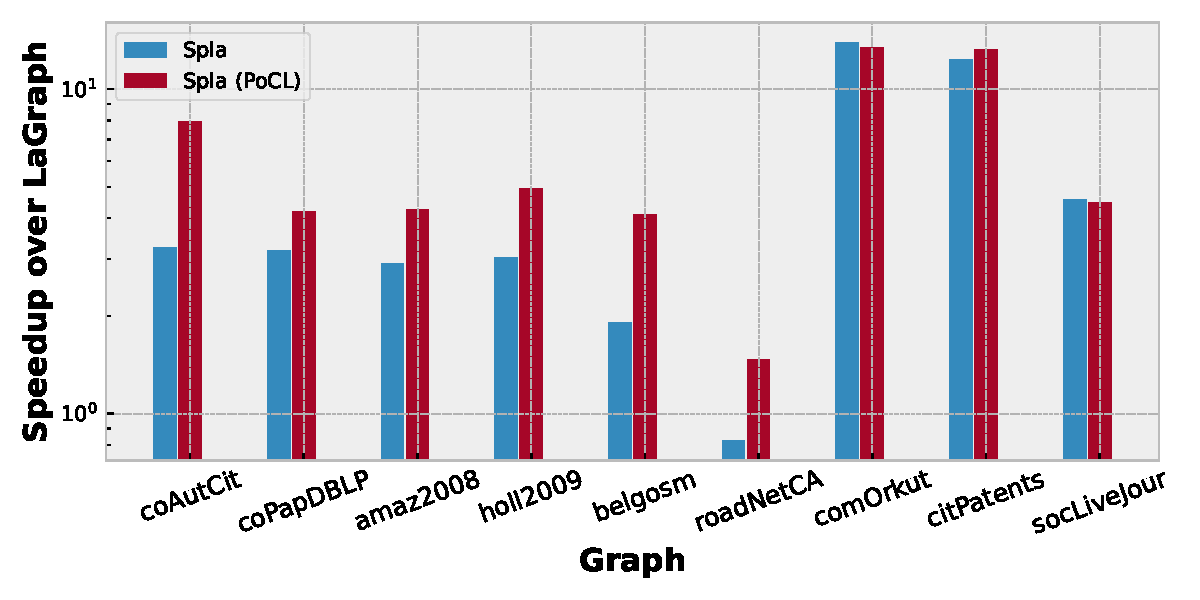
\includegraphics[width=0.9\linewidth]{pictures/rq1_rel_pr.pdf}
        \end{center}
    \end{columns}
    
\end{frame}

\begin{frame}
  \frametitle{Spla на ГПУ от Nvidia, Intel и AMD}
  \begin{center}
    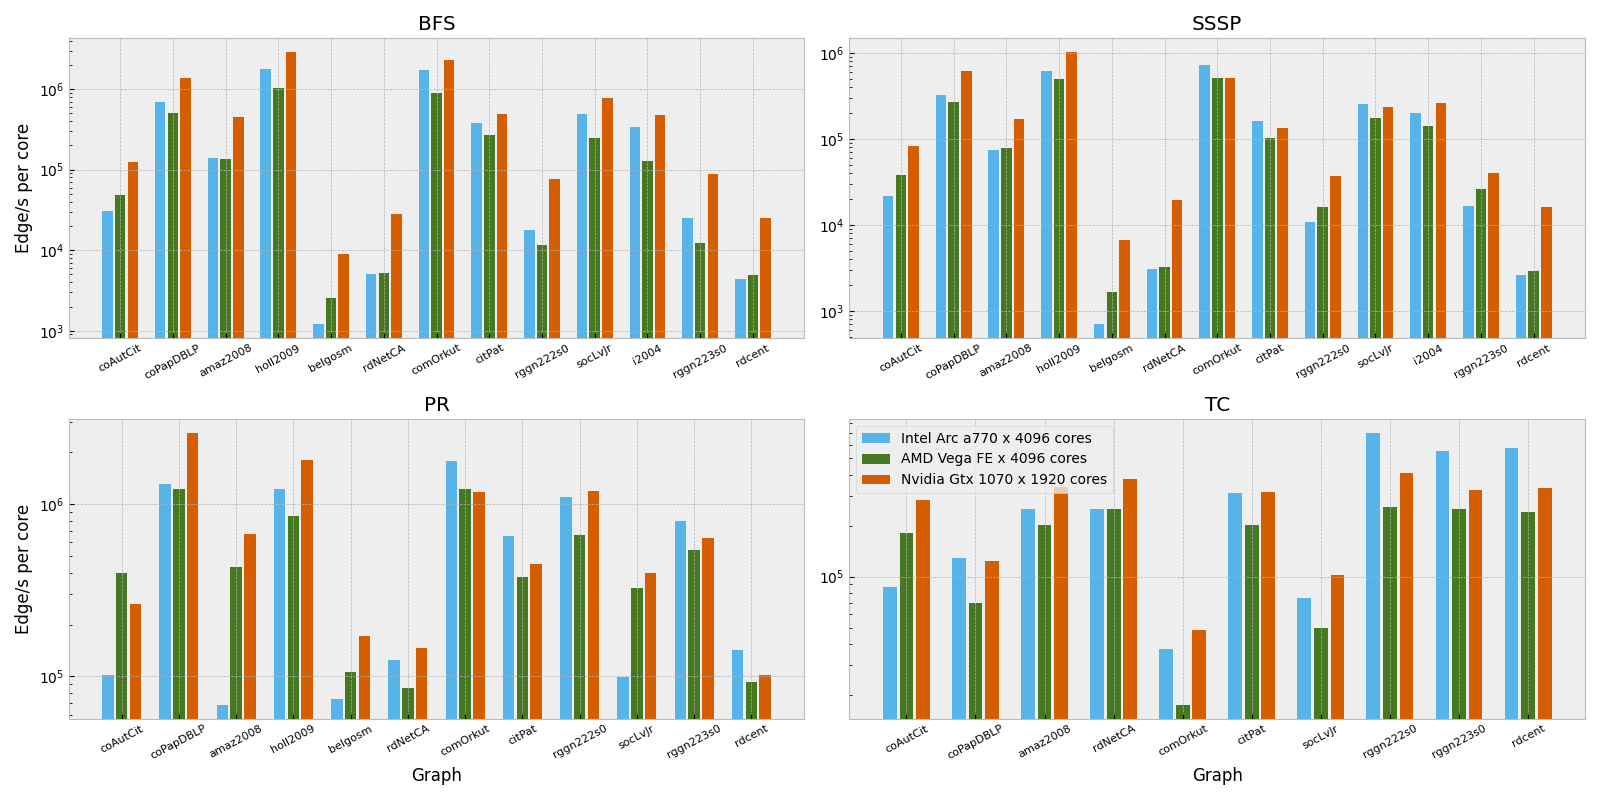
\includegraphics[width=0.95\linewidth]{pictures/rq2_cores.png}
  \end{center}
\end{frame}

\begin{frame}[fragile]
  \frametitle{Выводы}
  \begin{itemize}
    \item Есть решения для высокопроизводительного анализа графов с использованием линейной алгебры, пригодные для использования в экосистеме RISC-V 
    \begin{itemize}
      \item[\faCheck] CPU --- SuiteSparse:GpaphBLAS
        \begin{itemize}
          \item Стабильно работает, можно брать и пользоваться
          \item Требуются оптимизации\footnote{Впрочем, как и не на RISC-V}
        \end{itemize}
      \item[\faGears] GPGPGU --- Spla
      \begin{itemize}
          \item Многое работает, можно пробовать, ставить эксперименты
          \item Требуемая инфраструктура ``сырая'': не до конца отлажены драйвера, ``узкие'' PCI-шины, слабые ГПУ в доступных конфигурациях \ldots
      \end{itemize}
    \end{itemize}
    \item Нужны инструменты для профилирования
    \begin{itemize}
      \item В том числе, аппаратная поддержка (счётчики, \ldots)      
    \end{itemize}
  \end{itemize}
\end{frame}

\begin{frame}[fragile]
  \frametitle{Возможные направления}
  \begin{itemize}
    \item Проверка связок RISC-V CPU + AMD GPU и RISC-V CPU + Intel GPU
    \begin{itemize}
      \item Замеры Spla на них
    \end{itemize}
    \item Запуск работоспособных бенчмарок Spla на Vortex
    \item Эксперименты на более разнообразном ``железе''
    \item Анализ векторизации в SuiteSparse:GraphBLAS: что имеет смысл векторизовывать, какими средствами это лучше делать
    \item Исследование применимости матиричных расширений    
    \item Исследование производительности графовых СУБД на RISC-V
  \end{itemize}
\end{frame}

\appendix

\begin{frame}
  \frametitle{Результаты умножения плотных матриц на SpacemiT M1 с IMG GPU}
  \begin{center}
  \tikzmark{z1}{ }
  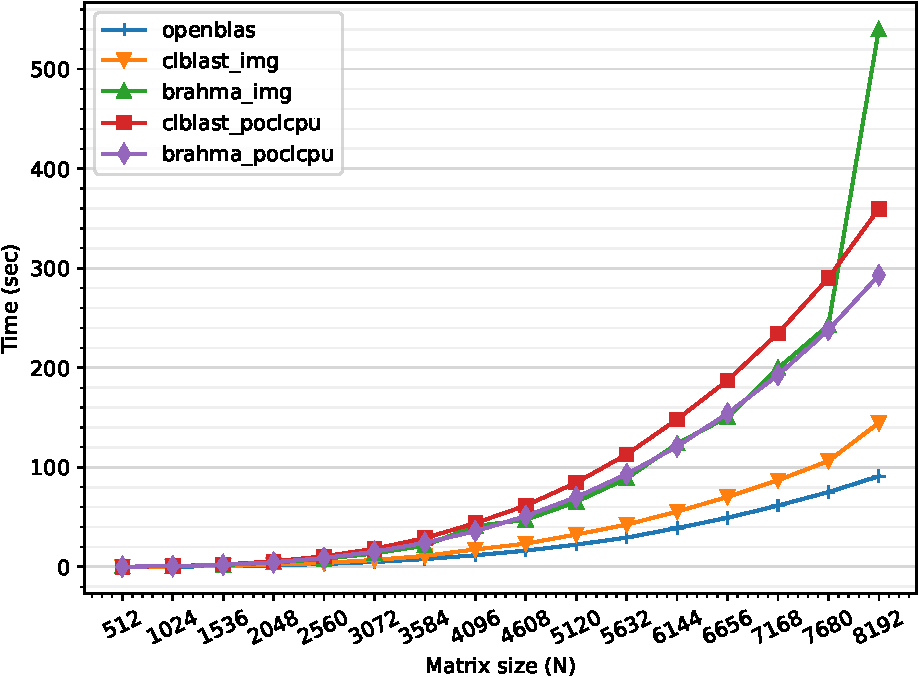
\includegraphics[width=0.55\textwidth]{pictures/MILK-V_crop.pdf}
  \tikz[overlay,remember picture]{\draw[draw=red,thick,double,fill opacity=0.2] ($ (z1) + (1.1,5.45)$) rectangle ($ (z1) + (3.4,6.05)$);}
  \\
    (Некоторые) GPGPU от Imagination Technologies (пока) не совсем для вычислений
  \end{center}
\end{frame}

\end{document}
